% =================================================
% MAIN DOCUMENT (NOTES TEMPLATE)
% =================================================
%
% Long-form theoretical physics and mathematics notes.
%
% Typographic appearance is defined in notesstyle.sty
% and should not be altered here.
%
% =================================================


\documentclass[a4paper,11pt]{article}


% =================================================
% LOAD NOTES STYLE
% =================================================
\usepackage{notesstyle}


% =================================================
% LANGUAGE
% =================================================
\usepackage[english]{babel}


% =================================================
% CUSTOM PACKAGES
%
% Add project-specific packages here.
% Do not insert packages elsewhere in the file.
% =================================================

% --- Mathematics (defaults) ---
% amsthm and the theorem/definition/remark environments
% are provided by notesstyle.sty.
\usepackage{amsmath, amssymb}
\usepackage{mathtools}

% --- Optional physics / math extensions ---
% \usepackage{physics}              % \dd, \ket, \bra, \comm, ...
% \usepackage{bm}                   % bold math symbols
% \usepackage{slashed}              % Feynman slash
% \usepackage{tensor}               % indexed tensors

% --- Other ---
\usepackage{graphicx}               % figures
\graphicspath{{figures/}}           % figures live in figures/
\usepackage{booktabs}               % tables
% \usepackage{enumitem}             % list customization


% =================================================
% CUSTOM COMMANDS
%
% Project-specific macros.
% =================================================

% \newcommand{\dd}{\mathrm{d}}
% \newcommand{\ii}{\mathrm{i}}


% =================================================
% METADATA
% =================================================
\title{Notes Title}
\author{Author Name}
\date{\today}


% =================================================
% DOCUMENT
% =================================================
\begin{document}

\maketitle

\begin{abstract}
These notes develop a small piece of theoretical machinery and
work through its consequences in detail. The exposition is kept
self-contained, with definitions, statements, short proofs, and
worked examples interleaved with prose. The closing sections
collect a few exercises for practice.
\end{abstract}

\clearpage
\framedtoc
\clearpage


% =================================================
\section{Setting}

These notes develop a small piece of theoretical machinery to
illustrate the structure of the template. The exposition follows
the typical pattern of mathematical and physics notes: definitions,
statements of results, short proofs, and worked examples interleaved
with prose.

Citations are rendered in brackets, e.g.\ \cite{example-article}, and
multiple sources combine and compress to ranges
automatically~\cite{example-article,example-book}.


% =================================================
\section{Definitions and Statements}

\begin{definition}
  Let $\mathcal{H}$ be a complex separable Hilbert space. A
  \emph{state} is a unit vector $\psi \in \mathcal{H}$, considered
  up to a phase factor $e^{i\theta}$.
\end{definition}

\begin{definition}
  An \emph{observable} is a self-adjoint linear operator $\hat{A}$
  acting on $\mathcal{H}$.
\end{definition}

The expectation value of an observable in a given state is defined by
\begin{equation}
  \langle A \rangle_\psi
  = \langle \psi | \hat{A} | \psi \rangle .
  \label{eq:expectation}
\end{equation}

\begin{theorem}
  Expectation values of self-adjoint operators are real.
\end{theorem}

\begin{proof}
  By definition,
  $\overline{\langle A \rangle_\psi}
  = \overline{\langle \psi | \hat{A} | \psi \rangle}
  = \langle \psi | \hat{A}^\dagger | \psi \rangle
  = \langle \psi | \hat{A} | \psi \rangle
  = \langle A \rangle_\psi$,
  where we used $\hat{A}^\dagger = \hat{A}$.
\end{proof}

\begin{remark}
  The reality of expectation values is what makes self-adjoint
  operators the natural mathematical model of observable quantities
  in quantum mechanics.
\end{remark}

\subsection{Time Evolution}

Time evolution in quantum mechanics is governed by the
Schr\"odinger equation:
\begin{equation}
  i\hbar \frac{\partial \psi}{\partial t}
  = \hat{H}\psi ,
  \label{eq:schrodinger}
\end{equation}
where $\hat{H}$ is the Hamiltonian. For time-independent
$\hat{H}$, equation~\eqref{eq:schrodinger} integrates to
\begin{equation}
  \psi(t) = e^{-i\hat{H}t/\hbar}\,\psi(0).
\end{equation}

\subsubsection{Stationary states}
A \emph{stationary state} is an eigenstate of $\hat{H}$; its time
dependence is a pure phase, so every expectation value is constant
in time. Run-in headings like this one mark the lowest structural
level and are kept out of the table of contents.


% =================================================
\section{Examples}

\begin{figure}[t]
  \centering
  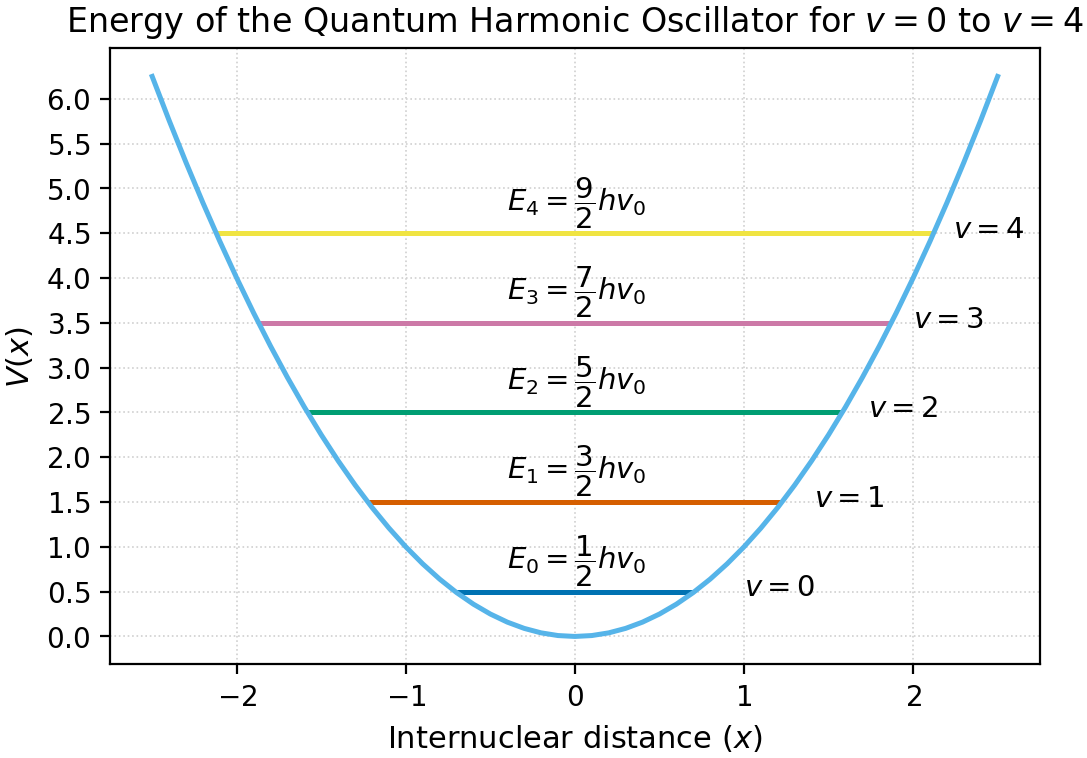
\includegraphics[width=0.7\linewidth]{Energy_levels}
  \caption{Schematic energy level diagram.}
  \label{fig:levels}
\end{figure}

Figure~\ref{fig:levels} shows a typical structure that recurs
throughout the rest of these notes. A few fundamental constants
are collected in Table~\ref{tab:constants} for reference.

\begin{table}[ht]
  \centering
  \caption{Fundamental physical constants.}
  \label{tab:constants}
  \begin{tabular}{lcr}
    \toprule
    Quantity            & Symbol  & Value                         \\
    \midrule
    Speed of light      & $c$     & $2.998 \times 10^8$ m/s       \\
    Planck's constant   & $\hbar$ & $1.055 \times 10^{-34}$ Js    \\
    Elementary charge   & $e$     & $1.602 \times 10^{-19}$ C     \\
    \bottomrule
  \end{tabular}
\end{table}


% =================================================
\section{Exercises}

Notes can carry problems alongside the exposition. The
\verb|exercise| environment is numbered per section and is
visually separated from the surrounding text by
\verb|\separator|. Subproblems use the \verb|subproblems|
environment, which labels parts a), b), c) without affecting
ordinary \verb|enumerate| lists.

\separator

\begin{exercise}
  Show that the eigenvalues of a self-adjoint operator
  $\hat{A}$ are real, and that eigenvectors belonging to
  distinct eigenvalues are orthogonal.
\end{exercise}

\begin{exercise}
  Consider a particle in a one-dimensional infinite square
  well of width $L$.
  \begin{subproblems}
    \item Write down the normalized energy eigenfunctions.
    \item Compute the energy levels $E_n$.
  \end{subproblems}

  The remaining parts build on the spectrum found above; use
  the result from part~(b) when sketching the densities.

  \begin{subproblems}[resume]
    \item Sketch the probability density for $n = 1, 2, 3$.
    \item Compute the expectation value $\langle x \rangle$ in
          the ground state.
  \end{subproblems}
\end{exercise}


% =================================================
\section{Closing}

These notes are a template; the content above exists only to
demonstrate typography. Replace it with your own material as the
notes develop.


% =================================================
% BIBLIOGRAPHY
% =================================================
\bibliographystyle{unsrtnat}
\bibliography{references}


\end{document}
